\documentclass[12pt]{report}
\usepackage[utf8]{inputenc}
\usepackage[russian]{babel}
%\usepackage[14pt]{extsizes}
\usepackage{listings}
\usepackage{graphicx}
\usepackage{amsmath,amsfonts,amssymb,amsthm,mathtools} 
\usepackage{pgfplots}
\usepackage{filecontents}
\usepackage{indentfirst}
\usepackage{eucal}
\usepackage{amsmath}
\usepackage{enumitem}
\frenchspacing

\usepackage{indentfirst} % Красная строка


%\usetikzlibrary{datavisualization}
%\usetikzlibrary{datavisualization.formats.functions}

\usepackage{amsmath}




% Для листинга кода:
\lstset{ %
language=haskell,                 % выбор языка для подсветки (здесь это С)
basicstyle=\small\sffamily, % размер и начертание шрифта для подсветки кода
numbers=left,               % где поставить нумерацию строк (слева\справа)
numberstyle=\tiny,           % размер шрифта для номеров строк
stepnumber=1,                   % размер шага между двумя номерами строк
numbersep=5pt,                % как далеко отстоят номера строк от подсвечиваемого кода
showspaces=false,            % показывать или нет пробелы специальными отступами
showstringspaces=false,      % показывать или нет пробелы в строках
showtabs=false,             % показывать или нет табуляцию в строках
frame=single,              % рисовать рамку вокруг кода
tabsize=2,                 % размер табуляции по умолчанию равен 2 пробелам
captionpos=t,              % позиция заголовка вверху [t] или внизу [b] 
breaklines=true,           % автоматически переносить строки (да\нет)
breakatwhitespace=false, % переносить строки только если есть пробел
escapeinside={\#*}{*)}   % если нужно добавить комментарии в коде
}

\usepackage[left=2cm,right=2cm, top=2cm,bottom=2cm,bindingoffset=0cm]{geometry}
% Для измененных титулов глав:
\usepackage{titlesec, blindtext, color} % подключаем нужные пакеты
\definecolor{gray75}{gray}{0.75} % определяем цвет
\newcommand{\hsp}{\hspace{20pt}} % длина линии в 20pt
% titleformat определяет стиль
\titleformat{\chapter}[hang]{\Huge\bfseries}{\thechapter\hsp\textcolor{gray75}{|}\hsp}{0pt}{\Huge\bfseries}


% plot
\usepackage{pgfplots}
\usepackage{filecontents}
\usetikzlibrary{datavisualization}
\usetikzlibrary{datavisualization.formats.functions}
\RequirePackage[
  style=gost-numeric,
  language=auto,
  autolang=other,
  sorting=none,
]{biblatex}

\addbibresource{bib.bib}
\begin{document}
%\def\chaptername{} % убирает "Глава"
\thispagestyle{empty}
\begin{titlepage}
	\noindent \begin{minipage}{0.15\textwidth}
	
\includegraphics[width=\linewidth]{b_logo}
	\end{minipage}
	\noindent\begin{minipage}{0.9\textwidth}\centering
		\textbf{Министерство науки и высшего образования Российской Федерации}\\
		\textbf{Федеральное государственное бюджетное образовательное учреждение высшего образования}\\
		\textbf{~~~«Московский государственный технический университет имени Н.Э.~Баумана}\\
		\textbf{(национальный исследовательский университет)»}\\
		\textbf{(МГТУ им. Н.Э.~Баумана)}
	\end{minipage}
	
	\noindent\rule{18cm}{3pt}
	\newline\newline
	\noindent ФАКУЛЬТЕТ $\underline{\text{«Информатика и системы управления»}}$ \newline\newline
	\noindent КАФЕДРА $\underline{\text{«Программное обеспечение ЭВМ и информационные технологии»}}$\newline\newline\newline\newline\newline
	
	
	\begin{center}
		\noindent\begin{minipage}{1.3\textwidth}\centering
			\Large\textbf{  Отчёт по лабораторной работе №5 по дисциплине}\newline
			\textbf{ "Методы машинного обучения"}\newline\newline
		\end{minipage}
	\end{center}
	
	\noindent\textbf{Тема} $\underline{\text{Байесовский классификатор <<Ирисов Фишера>>}}$\newline\newline
	\noindent\textbf{Студент} $\underline{\text{Варламова Е. А.}}$\newline\newline
	\noindent\textbf{Группа} $\underline{\text{ИУ7-23М}}$\newline\newline
	\noindent\textbf{Оценка (баллы)} $\underline{\text{~~~~~~~~~~~~~~~~~~~~~~~~~~~}}$\newline\newline
	\noindent\textbf{Преподаватели} $\underline{\text{Солодовников Владимир Игоревич}}$\newline\newline\newline
	
	\begin{center}
		\vfill
		Москва~---~\the\year
		~г.
	\end{center}
\end{titlepage}
\large
\setcounter{page}{2}
\def\contentsname{СОДЕРЖАНИЕ}
\renewcommand{\contentsname}{СОДЕРЖАНИЕ}
\tableofcontents
\renewcommand\labelitemi{---}
\newpage
\chapter{Теоретическая часть}

В 1936 году Рональд Фишер опубликовал статью, в которой он представил набор данных об ирисах, состоящий из трех различных видов: Iris setosa, Iris versicolor и Iris virginica. Для каждого вида ириса были измерены четыре характеристики: длина чашелистика, ширина чашелистика, длина лепестка и ширина лепестка.

Фишер использовал этот набор данных для демонстрации метода дискриминантного анализа, который позволяет разделить объекты на классы на основе их признаков. Он показал, что можно эффективно классифицировать ирисы по видам, используя комбинацию этих четырех признаков.

Ирисы Фишера стали одним из самых популярных наборов данных в машинном обучении и статистике. Они часто используются для тестирования алгоритмов классификации и кластеризации, а также для демонстрации методов визуализации данных.

Целью данной лабораторной работы является применение байесовского классификатора решения задачи классификации ирисов Фишера.
Для этого необходимо решить следующие задачи:
\begin{itemize}
    \item формализовать задачу;
    \item описать алгоритм байесовского классификатора;
    \item привести особенности реализации ПО, решающего поставленную задачу;
    \item оценить точность, полноту, F-меру. Построить матрицу ошибоки.
\end{itemize}

\section{Постановка задачи}

Построить классификатор <<Ирисов Фишера>> с использованием байесовского подхода.
В ходе выполнения работы:
\begin{enumerate}
    \item Осуществить исследование и подготовку исходных данных.
    \item Построить гистограммы распределения значений для каждого признака и для каждого класса.
    \item Произвести визуализацию проекций классов на плоскости, где по осям  отложены различные комбинации пар признаков.
    \item Построить матрицы корреляций между различными признаками, как для всей выборки в целом, так и для отдельных классов.
    \item Построить классификатор с использованием байесовского подхода.
    \item Оценить точность, полноту, F-меру. Построить матрицу ошибок.
\end{enumerate}

\section{Алгоритм наивного байесовского классификатора}
Классификация с использованием наивного байесовского классификатора основана на применении теоремы Байеса. Пусть дан набор объектов $X = (x_1, x_2, ..., x_n)$ и метки классов $Y = (y_1, y_2, ..., y_m)$. Наивный байесовский классификатор предполагает, что все признаки объектов независимы друг от друга при условии класса. Таким образом, вероятность принадлежности объекта x к классу y может быть вычислена по формуле:

\begin{equation}
  P(y|x) = P(x|y)P(y)/P(x)  
\end{equation}
    
где 
\begin{enumerate}
    \item $P(y|x)$ - вероятность принадлежности объекта $x$ к классу $y$;
    \item $P(x|y)$ - вероятность объекта $x$ при условии класса $y$;
    \item $P(y)$ - априорная вероятность класса $y$;
    \item $P(x) $- вероятность объекта $x$.
\end{enumerate}

Для наивного байесовского классификатора используются различные модели для оценки вероятностей $P(x|y)$ и $P(y)$. Например, для категориальных данных можно использовать модель мультиномиального распределения, а для непрерывных данных - модель нормального распределения.

На практике для классификации объекта выбирается класс с наибольшей вероятностью $P(y|x)$:

\begin{equation}
    y' = max_y \in Y P(y|x)
\end{equation}

где $y'$ - предсказанная метка класса для объекта $x$.

Таким образом, наивный байесовский классификатор является простым и эффективным методом классификации, основанным на принципах вероятностного вывода.


\chapter{Практическая часть}

\section{Выбор средств разработки}
В качестве языка программирования был использован язык Python, поскольку этот язык кроссплатформенный и для него разработано огромное количество библиотек и модулей, решающих разнообразные задачи. 

В частности, имеются библиотеки, включающие в себя алгоритм наивного байесовского классификатора  в библиотеке \cite{bib:scipy}.

\section{Исследование ПО}

В листинге \ref{lst:gen1} представлен код, решающий задачу классификации ирисов.

\begin{lstlisting}[label=lst:gen1,caption=Код классификации ирисов]
import pandas as pd
import numpy as np
import matplotlib.pyplot as plt
import seaborn as sns
from sklearn.model_selection import train_test_split
from sklearn.naive_bayes import GaussianNB
from sklearn.metrics import accuracy_score, precision_score, recall_score, f1_score, confusion_matrix

data = pd.read_csv('data.csv')

print(data.describe())
sns.pairplot(data, hue='iris_type', palette='husl')
plt.savefig("pairs.png")
plt.clf()

correlation_matrix = data.corr()
sns.heatmap(correlation_matrix, annot=True, cmap='coolwarm')
plt.title('Матрица корреляции для всех данных')
plt.savefig("whole_matrix.png")
plt.clf()

for iris_class in data['iris_type'].unique():
    subset = data[data['iris_type'] == iris_class]
    correlation_matrix = subset.corr()
    sns.heatmap(correlation_matrix, annot=True, cmap='coolwarm')
    plt.title(f'матрица корреляций для {iris_class}')
    plt.savefig(f"matrix_{iris_class}.png")
    plt.clf()


X = data.drop('iris_type', axis=1)
y = data['iris_type']

X_train, X_test, y_train, y_test = train_test_split(X, y, test_size=0.4, random_state=42)

model = GaussianNB()
model.fit(X_train, y_train)

y_pred = model.predict(X_test)

accuracy = accuracy_score(y_test, y_pred)
precision = precision_score(y_test, y_pred, average='weighted')
recall = recall_score(y_test, y_pred, average='weighted')
f1 = f1_score(y_test, y_pred, average='weighted')
conf_matrix = confusion_matrix(y_test, y_pred)



sns.heatmap(conf_matrix, annot=True)
plt.title(f'acc={accuracy:.2f}, prec={precision:.2f}, Recall={recall:.2f}, f1={f1:.2f}')
plt.savefig(f"matrix_errors.png")
plt.clf()
\end{lstlisting}

\newpage
С помощью разработанного ПО были построены гистограммы распределения значений для каждого признака и для каждого класса (по диагонали), а также произведена визуализация проекций классов на плоскости, где по осям  отложены различные комбинации пар признаков на рисунке \ref{fig:pairs}. 

\begin{figure}[h!]
  \centering
  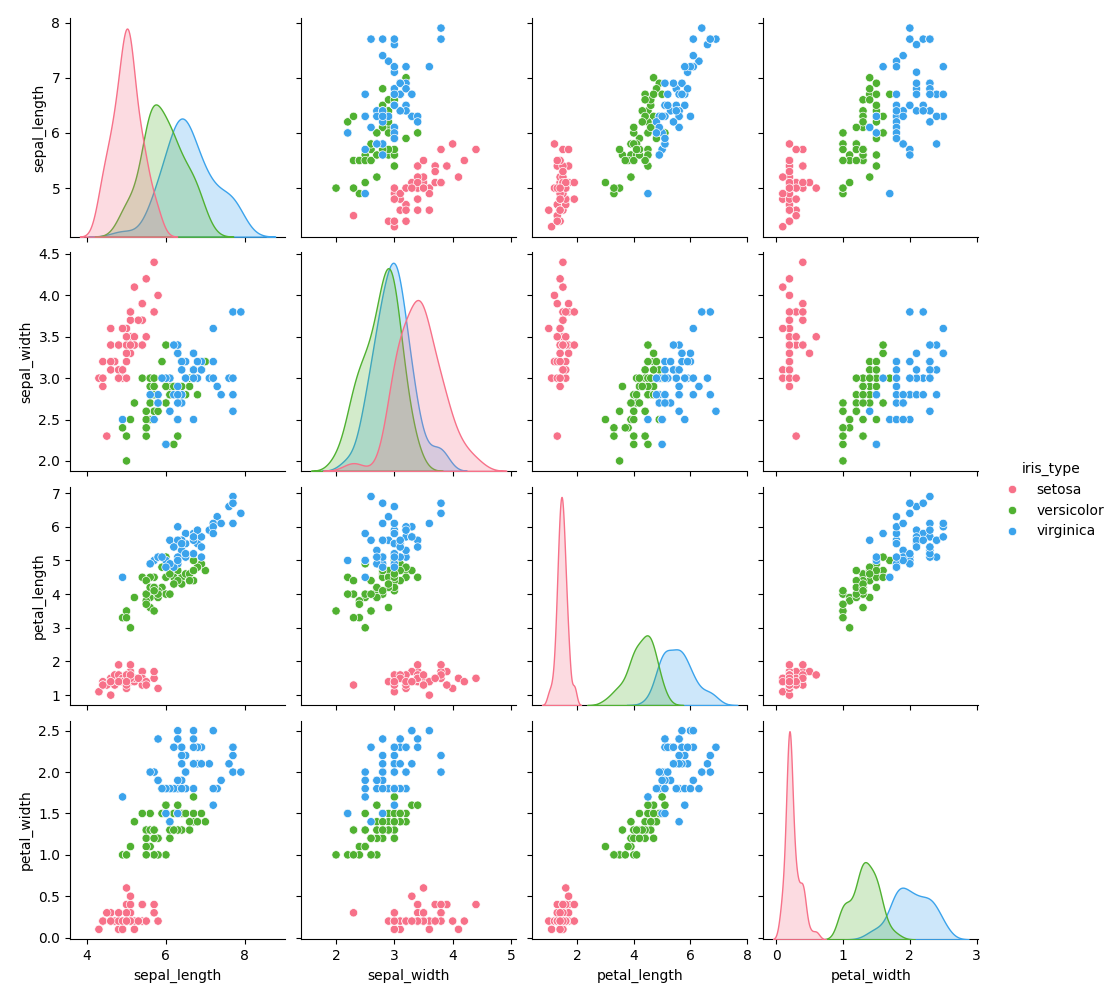
\includegraphics[width = \linewidth]{pairs.png}
  \caption{Гистограммы распределения и проекции классов для пар признаков}
  \label{fig:pairs}
\end{figure}

По рисунку видно, что распределения всех признаков классов близки к нормальным, при этом с разными параметрами закона, что говорит о возможности разделения классов (например, если у одного класса среднее значение признака выше, чем у другого класса, это может быть важным признаком для разделения классов). Аналогично, по проекциям классов на плоскости для пар признаков можно сделать вывод, что данные хорошо разделяются на классы. 


Также были построены матрицы корреляций между различными признаками на рисунке \ref{fig:whole}, как для всей выборки в целом, так и для отдельных классов \ref{fig:setoza}-\ref{fig:virginica}.

\begin{figure}[h!]
  \centering
  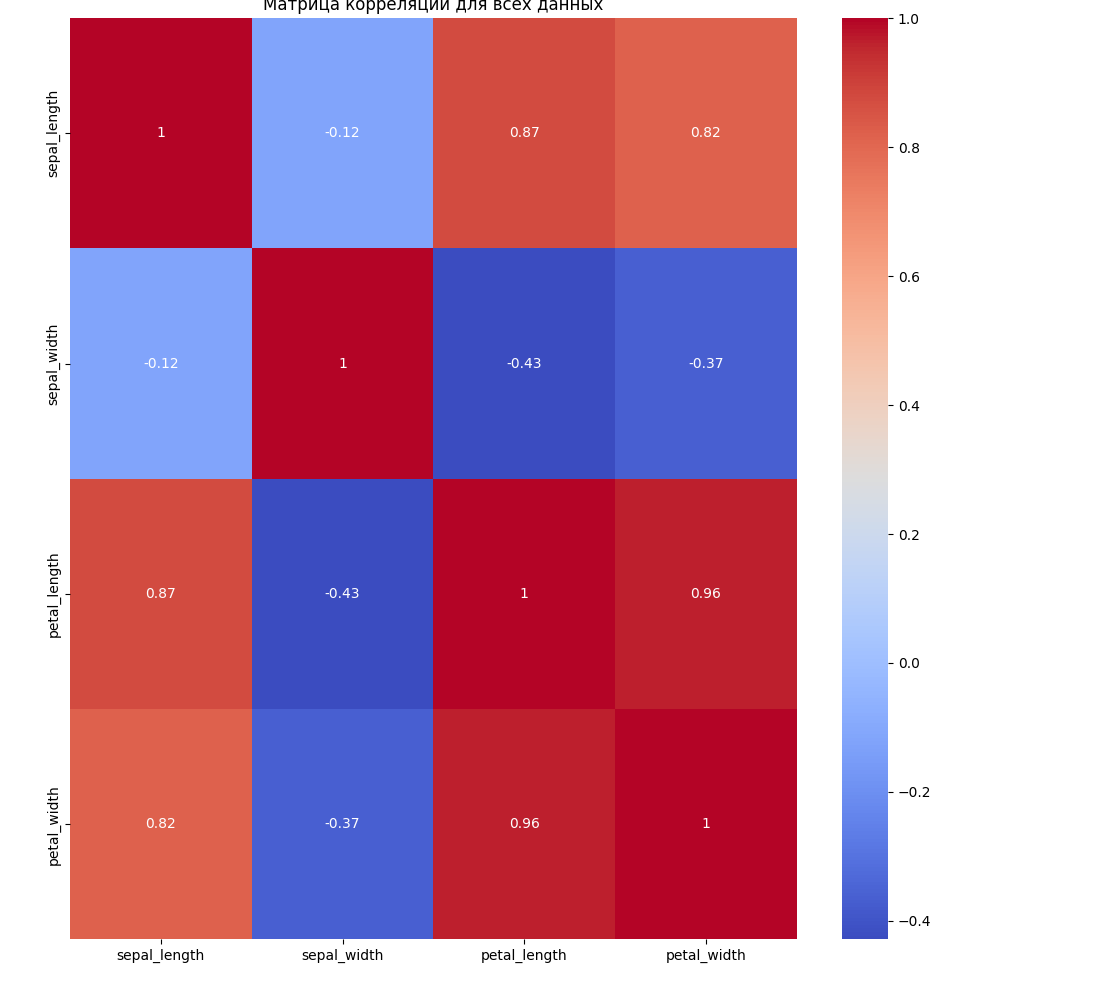
\includegraphics[width = \linewidth /2]{whole_matrix.png}
  \caption{матрица корреляций для всей выборки}
  \label{fig:whole}
\end{figure}

\begin{figure}[h!]
  \centering
  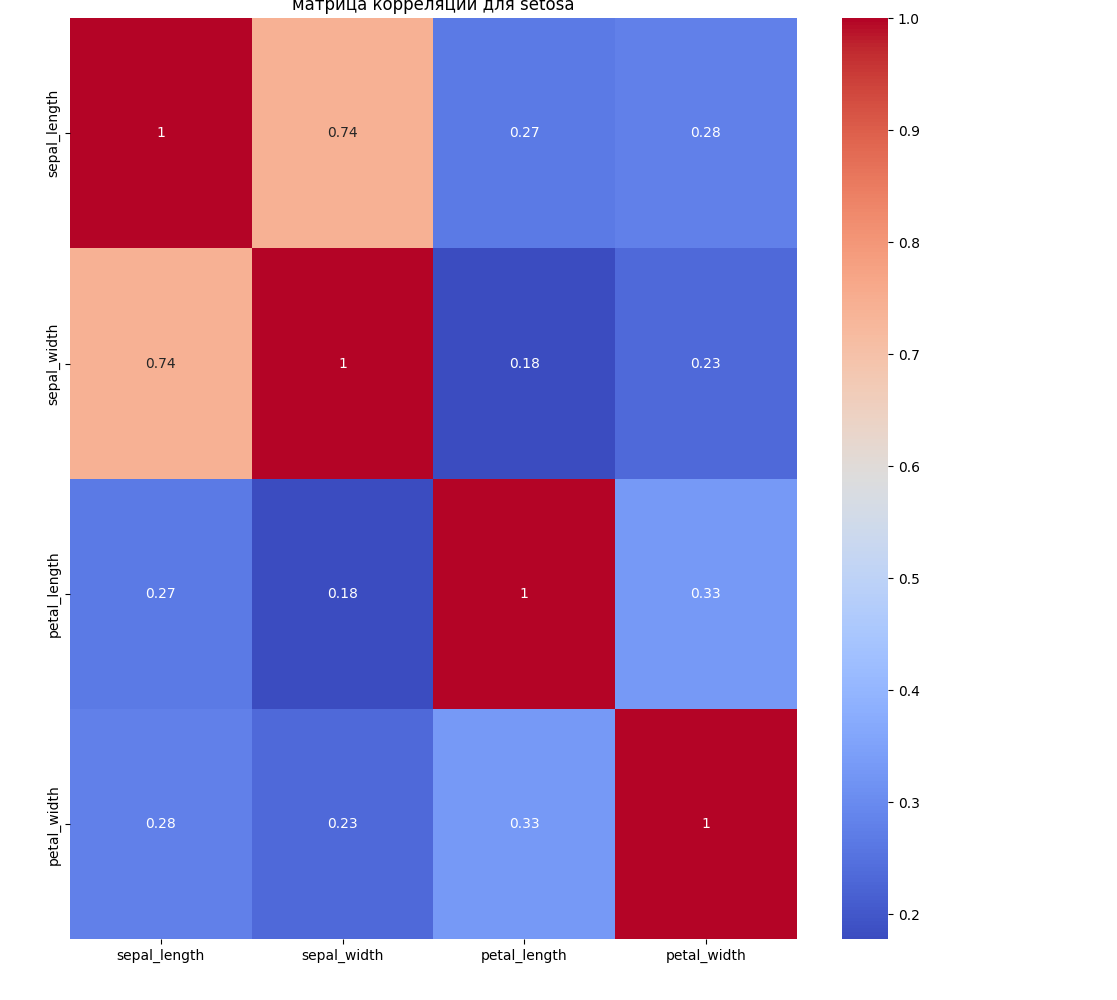
\includegraphics[width = \linewidth /2]{matrix_setosa.png}
  \caption{матрица корреляций для setoza}
  \label{fig:setoza}
\end{figure}

\begin{figure}[h!]
  \centering
  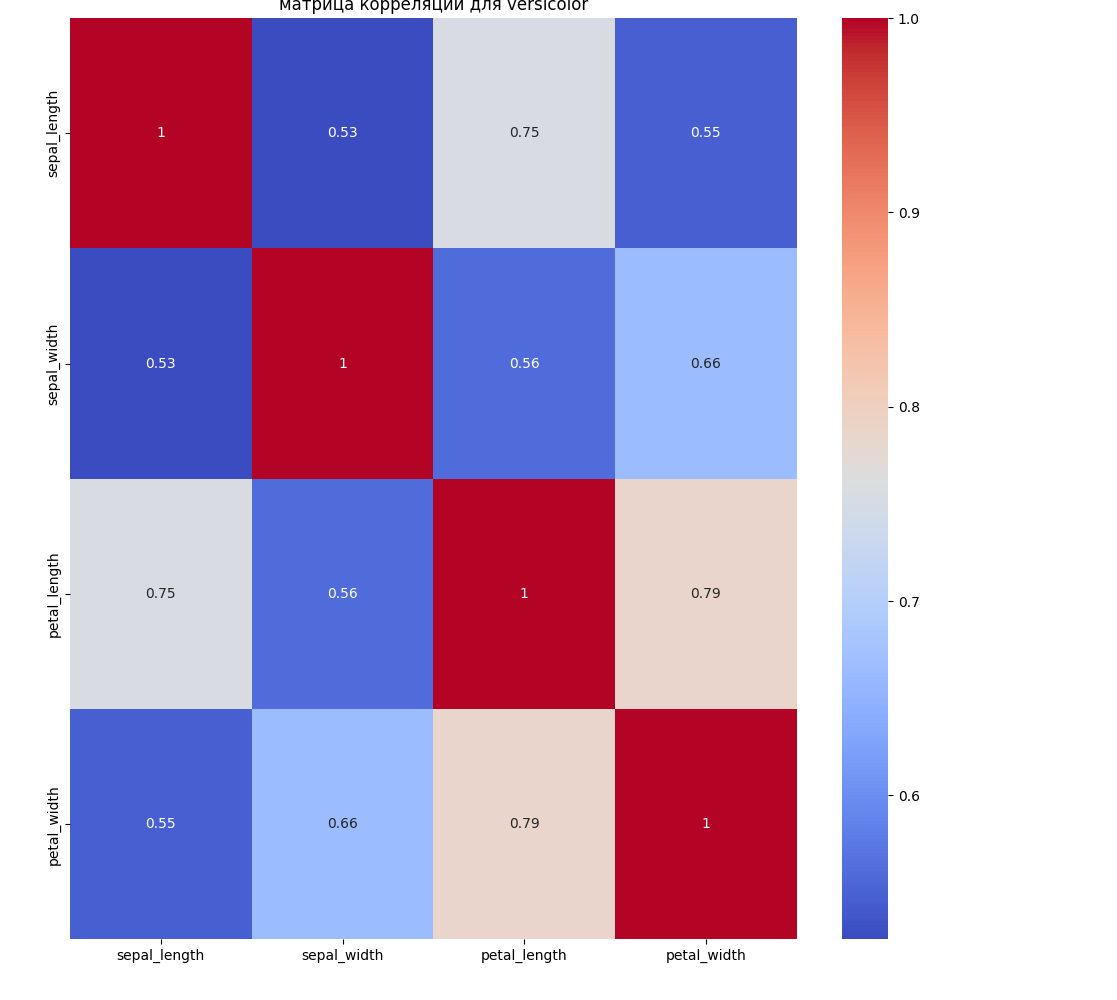
\includegraphics[width = \linewidth /2]{matrix_versicolor.png}
  \caption{матрица корреляций для versicolor}
  \label{fig:versicolor}
\end{figure}

\begin{figure}[h!]
  \centering
  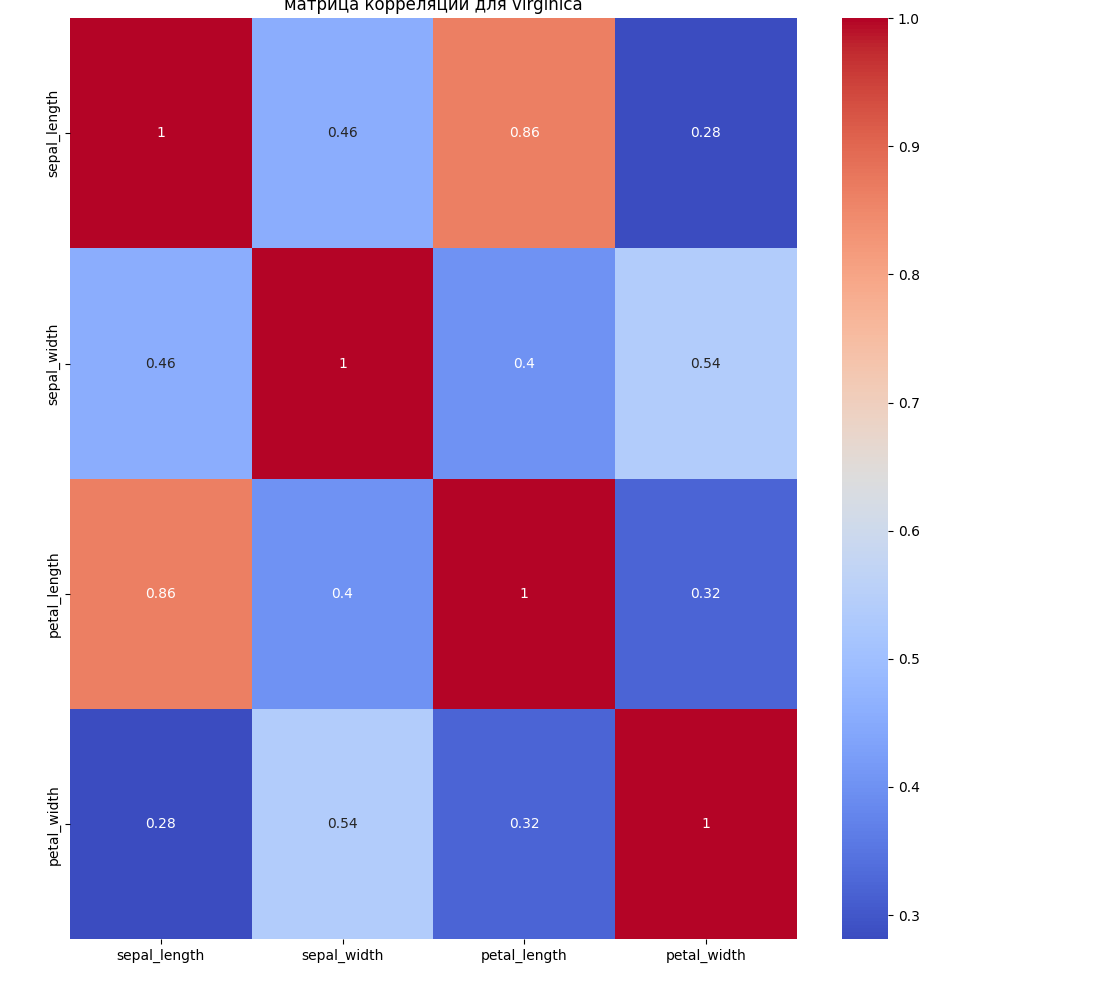
\includegraphics[width = \linewidth /2]{matrix_virginica.png}
  \caption{матрица корреляций для virginica}
  \label{fig:virginica}
\end{figure}

\newpage
Видно, что в большинстве классов наблюдается слабая корреляция между признаками. 
\newpage

Также была оценена точность, полнота, F-мера и построена матрица ошибки после классификации.

При разделении данных в пропорции 6:4 (обучающая:тестовая) были получены следующие результаты (рисунок \ref{fig:errors}).

\begin{figure}[h!]
  \centering
  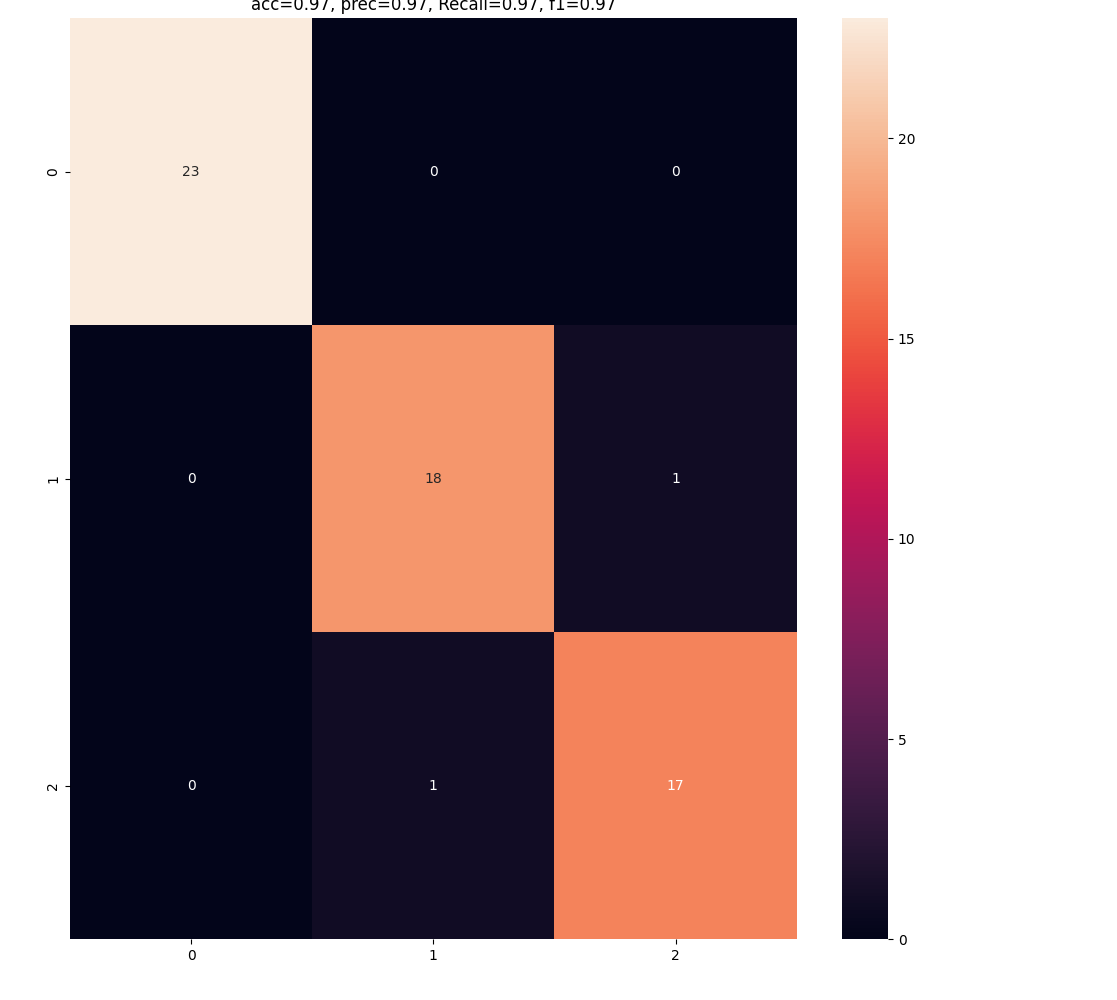
\includegraphics[width = \linewidth ]{matrix_errors.png}
  \caption{матрица ошибок}
  \label{fig:errors}
\end{figure}

\begin{itemize}
    \item Accuracy: 0.97;
    \item Precision: 0.97;
    \item Recall: 0.97;
    \item F-мера: 0.97 .
\end{itemize}
\newpage
При разделении данных в пропорции 8:2 (обучающая:тестовая) были получены следующие результаты (рисунок \ref{fig:errors_2}).

\begin{figure}[h!]
  \centering
  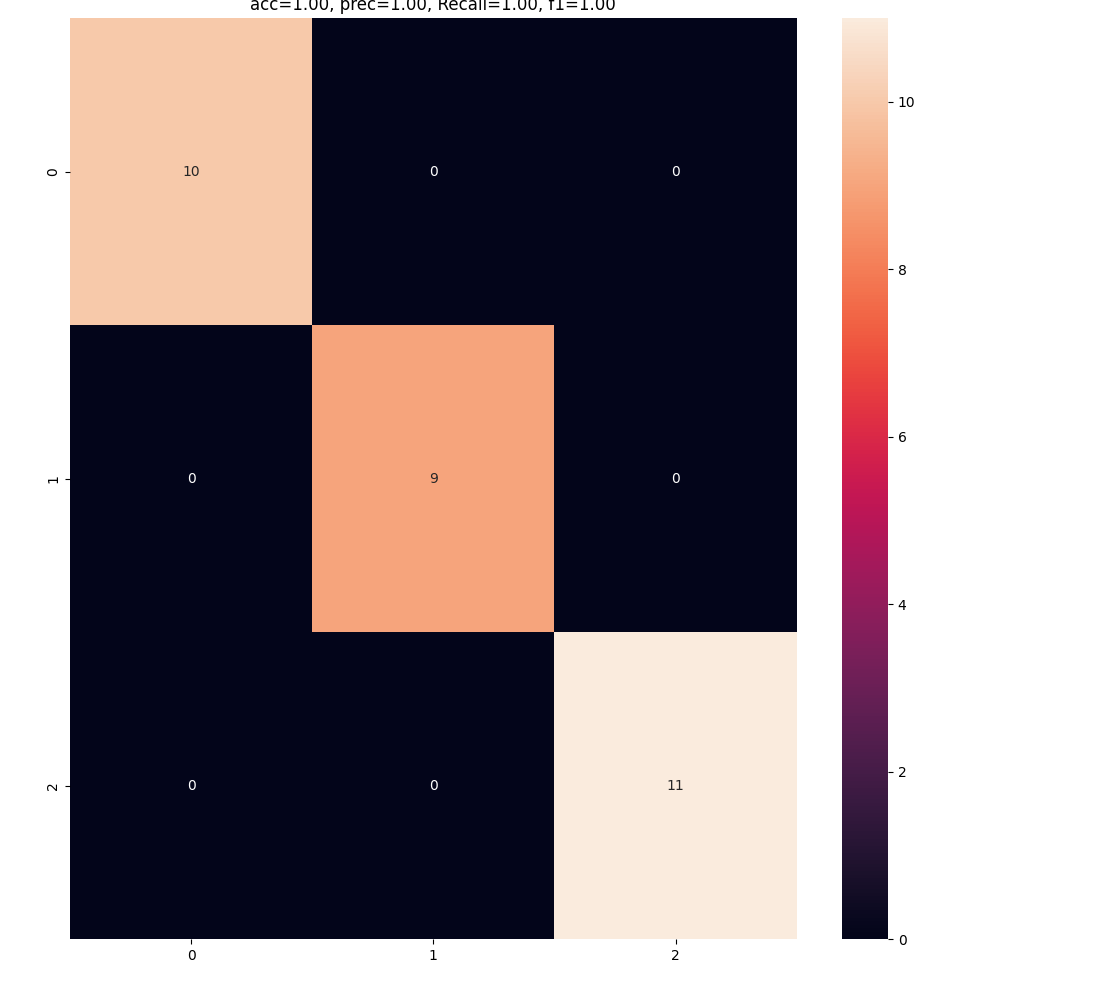
\includegraphics[width = \linewidth ]{matrix_errors_2.png}
  \caption{матрица ошибок}
  \label{fig:errors_2}
\end{figure}

\begin{itemize}
    \item Accuracy: 1;
    \item Precision: 1;
    \item Recall: 1;
    \item F-мера: 1 .
\end{itemize}

Таким образом, классификация была проведена абсолютно точно при разделении 8:2 и с ошибкой в 3\% при разделении 6:4.

\printbibliography[title={СПИСОК ИСПОЛЬЗОВАННЫХ\\ ИСТОЧНИКОВ}]
\addcontentsline{toc}{chapter}{СПИСОК ИСПОЛЬЗОВАННЫХ ИСТОЧНИКОВ}

\end{document}